\documentclass{article}
\usepackage{pythonhighlight}
\usepackage{graphicx}
\usepackage{ctex}
\usepackage[left=3cm,top=3cm,right=3cm]{geometry}
\usepackage{hyperref}
% TITLE PAGE CONTENT %%%%%%%%%%%%%%%%%%%%%%%%
%%%%%%%%%%%%%%%%%%%%%%%%%%%%%%%%%%%%%%%%%%%%%
\newcommand{\labno}{03}
\newcommand{\labtitle}{EE208 Crawler}
\newcommand{\authorname}{周李韬}
\newcommand{\studentno}{518030910407}
\newcommand{\classno}{F1803016}
% END TITLE PAGE CONTENT %%%%%%%%%%%%%%%%%%%%


\begin{document}

\begin{center}
{\LARGE \textsc{Laboratory No. \labno:} \\ \vspace{4pt}}
{\Large \textsc{\labtitle} \\ \vspace{4pt}} 
\rule[13pt]{\textwidth}{1pt} \\ \vspace{15pt}
{\large By: \authorname \\ \vspace{10pt}
No. \studentno \\ \vspace{10pt}
SJTU \classno \\ \vspace{10pt}
\today \vspace{20pt}}
\end{center}



\section{实验准备}

\subsection{实验环境}
\begin{itemize}
\item\textbf{Environment} Ubuntu 16.04 (on Virtual Machine)
\item\textbf{Language} Python 2.7.16 with packages as follows
	\begin{itemize}
	\item urllib 1.24.2
	\item beautifulsoup4 4.8.0
	\end{itemize}
\item\textbf{Tools} PyCharm 2019.2, Virtual Box
\end{itemize}
Python脚本在Windows 10上也通过了测试.

\subsection{实验目的}
本实验分为两个部分,在第一部分,我们要实现一个简单的BloomFilter。第二部分中,我们要在上一次crawler实验的基础上,实现一个并行式的crawler。

\subsection{实验原理}
\label{sec:principle}

在爬虫的遍历图算法中,我们需要有一个集合来记录已经爬过的网页,如果采用线性表等方式存储将会极大增加时间复杂度。为此我们采用BloomFilter的方法。BloomFilter的本质是一个BitMap,每一个URL会通过若干哈希函数映射到BitMap的若干对应位中,如果这些位数都已被标记过,我们就“认为”当前URL已经在BloomFilter中。实验源代码中已提供了一个Bitarray的实现,本实验的第一部分,将在该Bitarray类的基础上,增加与BloomFilter相关的成员函数。

为提高爬虫的效率,我们可以将Lab2中的爬虫改为并行式的实现。我们的实现思路是将Lab2 Crawler中的tocrawl队列作为任务队列,每一个线程都从该任务队列中获取新的任务,对该page做保存、提取页面中的URL、添加到tocrawl队列中的操作。同时我们设置一个全局计数器,统计已爬网页的个数,当达到预先设定的max\_page时,清空队列,结束多线程。

此外,我还做了将第一部分的BloomFilter嵌入第二部分的并行化爬虫的工作。以上是两部分实验的基本原理,它们具体的实现将会在下文展开。

\section{实验步骤}
\subsection{Exercise 1}


\subsubsection{Solution}
我们需要在Bitarray中增加以下功能:
\begin{enumerate}
\item 输入一个字符串,返回它的哈希映射列(通过若干哈希函数生成)
\item 输入一个字符串或它的哈希映射列,在Bitarray中添加该字符串的标记
\item 输入一个字符串或它的哈希映射列,判断Bitarray中是否存在
\end{enumerate}

我们采用类的成员函数的方式实现。具体实现方式如下:

\paragraph{字符串的哈希映射列}
在本实验中,我们采用同一个哈希函数BKDRHash,给定十个不同的种子,生成了一个长度为10的哈希映射列。实验源代码中已给了BKDRHash函数的实现,我们做了一些修改,在函数中加了一个种子参数,方便get\_hashstr函数中,赋予不同种子值时的循环调用。其中get\_hashstr的种子列表hash\_seed可以被随意修改。代码如下。
\begin{python}
def get_hashstr(self, keyword):
    """ return a 10-bit hash string for a string """
    res = []
    hash_seed = [31, 133, 1245, 4, 683, 235, 986, 1325, 8539, 4452]
    for j in range(10):
        res.append(self.BKDRHash(hash_seed[j], keyword) % self.size) 
                   # 将哈希映射结果取Bitarray大小的余数,达到平均映射的效果
    return res

def BKDRHash(self,seed, key):
    """ a BKDRHash function where seed can be set manually """
    hash = 0
    for i in range(len(key)):
        hash = (hash * seed) + ord(key[i])
    return hash
\end{python}

\paragraph{判断字符串是否在BloomFilter中}
为方便不同情形下的使用,我们写了两个判断函数,分别用于判断字符串或者字符串的哈希映射列是否在BloomFilter中。具体实现而言,我们“认为”一个字符串在BloomFilter中的标准是它的所有哈希映射值都被标记过,在Bitarray中,已经有了判断一个值是否在哈希表中的函数实现,对一个十位的哈希映射列,我们就调用十次Bitarray.get()函数,取十个布尔值的交,那么最终返回值只有在十位全部被标记过时才会为真,符合我们判别的要求。代码如下。
\begin{python}
def has_hashstr(self, hstr):
    """ Match the hstr with the bitarray, return true if all matched """
    res = True
    for i in hstr:
        res = (res and self.get(i))
    return res

def has_str(self, str):
    """ Match the string with the bitarray, return true if all matched """
    strhash = self.get_hashstr(str)
    return self.has_hashstr(strhash)
\end{python}

\paragraph{将字符串加入BloomFilter中}
类似地,为方便不同情形下的使用,我们写了两个add函数,分别用于添加字符串或者字符串的哈希映射列到BloomFilter中。Bitarray类中已经有了将一个值加入Bitarray标记的set函数,我们在哈希映射列中循环调用该函数,可达到字符串写入的效果。
\begin{python}
def add_str(self, str):
    """ Add the str into the bitarray """
    strhash = self.get_hashstr(str)
    self.add_hashstr(strhash)
    return 0

def add_hashstr(self, strhash):
    for i in strhash:
        self.set(i)
    return 0
\end{python}


\subsubsection{Test}
如图\ref{fig:flowchart}所示,BloomFilter的建立和测试流程如下。测试集我们采用了公版电子书“The Adventures of Sherlock Holmes”,首先我们对该文本进行了去重处理(见textprocessing.py),将去重后的文档(test.txt)每一行看做一个字符串,用于BloomFilter的测试。每一次测试中,我们首先获取当前行的哈希映射列,进而检查它是否已“存在”在BloomFilter中,由于已经过去重处理,因此凡是“存在”的情况都表明BloomFilter出现了混淆的情况,因此将该行的输入标记为false positive。最后通过统计false positive的出现次数,我们可以检验BloomFilter的可靠性。


\begin{figure}[htbp]
\centering
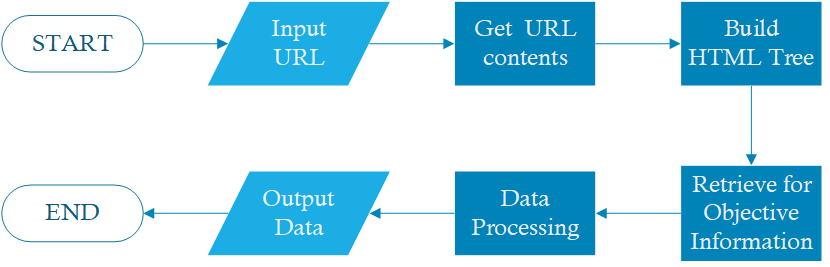
\includegraphics[width=9.5cm]{img/flowchart.png}
\label{fig:flowchart}
\caption{BloomFilter的测试流程}
\end{figure}

\subsubsection{Results}
测试的结果图\ref{img:1}所示:


测试表明,对我们采用的测试集,当我们取10个哈希函数,位数组大小为200000,大约为字符串个数的20倍时,10003行数据中出现了7次false positive,发生概率约为万分之七,与\href{http://pages.cs.wisc.edu/~cao/papers/summary-cache/node8.html}{BloomFilters-the math}的结论相符,表明我们搭建的BloomFilter基本能满足爬虫的需求。进一步,当位数组大小提高到700000时,对该测试集则没有false positive出现了。

\begin{figure}[htbp]
\centering
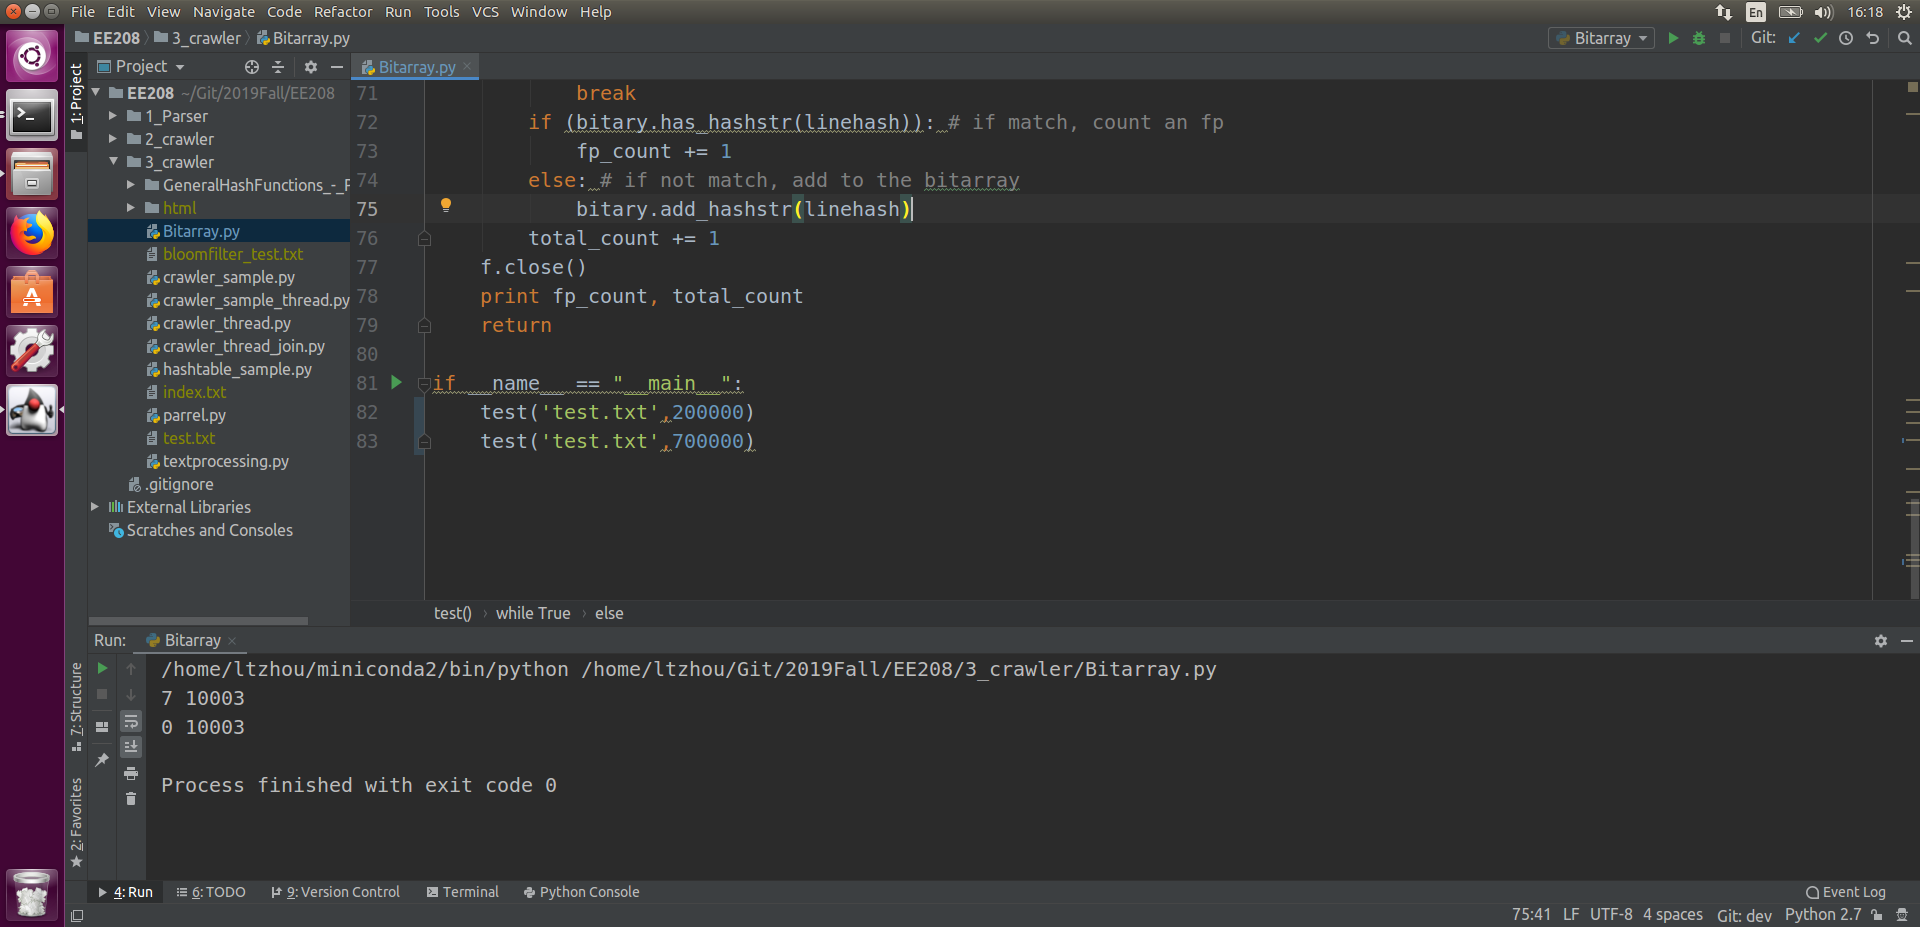
\includegraphics[width=13.5cm]{img/test1.png}
\caption{BloomFilter Testing}
\label{img:1}
\end{figure}

\subsection{Exercise 2}

\subsubsection{Solution}

在该部分实验中,我们需要将Lab2中的爬虫改为并行式。

\paragraph{多线程实现}
要将原本单线程运行的crawler改成并行式,我们需要做以下工作。

首先,我们将待爬取的队列改为一个工作队列,Python中Queue库可以提供这一功能,且其中的task\_done等函数可以保证多线程运行时的锁安全性。每一个队列中的URL都代表了一个任务,每个线程运行时,会从Queue中获得一个URL,完成操作后,将这一任务结束。

其次,对于线程间公用的数据,如已被爬取的URL集合crawled、已爬取的网站计数器COUNT、图结构graph,以及最初传入的参数,如种子网页seed、目标爬取网页数max\_page、线程数NUM等,我们需要将其设置为全局变量。

接下来,我们根据用户设定的线程NUM,建立相应的线程。建立代码如下:

\begin{python}
threads =[]                   # 线程列表
for i in range(NUM):
    t = threading.Thread(target=page_working)
                              # 每一个线程中,执行page_working函数
    t.setDaemon(True)         # 线程被设置为守护进程,随着主线程的退出而退出
    threads.append(t)         # 将线程加入线程列表中,方便管理
for t in threads:
    t.start()                 # 开始线程
\end{python}

对每一个线程具体的工作,将在page\_working函数中进行实现。我们为page\_working函数设置了退出条件,保证每一个线程会在总爬取数大于预设值时退出。在主函数中,我们用join函数等待子线程的完成,即可完成主程序的退出。

\begin{python}
for t in threads:
    t.join()
\end{python}

\paragraph{工作函数}
根据前文的设定,我们的工作函数需要从队列中获取新的URL任务,爬取存储网页内容、提取该页面上的所有URL并加入接下来的队列中。此外,当已爬取的页面大于设定时,结束循环。工作函数与单线程爬虫基本类似,不同之处在于此处我们在往工作队列添加新的URL时,需要用队列的方法(即union函数),其本质是与BFS一致的。以下的代码为不带变量锁时的工作函数。

\begin{python}
def page_working():
    while (COUNT < int(max_page)):
        page = tocrawl.get()        # 从工作队列获取URL
        if crawled.has_str(page):   # 若URL未被访问过
            print page
            content = get_page(page)
            if content:             # 保存网页信息、获取网页中的URL
                add_page_to_folder(page, content)
                outlinks = get_all_links(content, page)
                union(tocrawl, outlinks)
                crawled.add_str(page)
                graph[page] = outlinks
                COUNT += 1
        tocrawl.task_done()         # 队列中完成当前任务
def union(a,b):
    for e in b:
        a.put(e)
\end{python}

\paragraph{Crawled集合的BloomFilter实现}
在本部分实验中,我们可以将前一部分实验中构造的BloomFilter加入其中,根据此前的实验结果,我们采用20倍max\_page长度的BitMap用于创建crawled对象。在工作函数中,我们可以直接调用Bitarray类中的has\_str()函数作为当前页面是否被访问过的条件判断,调用add\_str()函数作为将新访问的页面加入crawled集合的操作实现。在主函数中的创建crawled实例的代码如下,工作函数中的crawled成员函数的调用可见上一段代码。

\begin{python}
from Bitarray import Bitarray

seed = 'http://www.163.com'
max_page = 100
crawled = Bitarray(20*max_page)
\end{python}

\paragraph{变量锁}
在多线程中,同时操作全局变量将造成不必要的冲突和麻烦,为此我们在操作全局变量时加上变量锁。varLock是我们在主函数中建立的一个thread库中的Lock实例。注意到工作函数中,判断条件中涉及了全局变量COUNT,因此加变量锁时,我们改用break结构,将判断放入函数体中,方便我们能在涉及全局变量时,统一进行变量锁的操作。我们最终版本的工作函数代码如下。
\begin{python}
def page_working():
    global COUNT
    while (True):
        page = tocrawl.get()
        if varLock.acquire():   # ---- begin of varlock -----
            has_str = crawled.has_str(page)
                           # has_str是一个确认当前页面是否被访问过的布尔值
            if (COUNT>=max_page):
                varLock.release()
                break      # 退出条件
            varLock.release()   # ----- end of varlock ------
        if (not has_str):
            print COUNT,page
            content = get_page(page)
            if content:    # 保存网页信息、获取网页中的URL
                crawled.add_str(page)
                add_page_to_folder(page, content)
                outlinks = get_all_links(content, page)
                if varLock.acquire():  # -- begin of varlock --
                    union(tocrawl, outlinks)
                    graph[page] = outlinks
                    COUNT += 1
                    varLock.release()  # --- end of varlock ---
        tocrawl.task_done()    # 队列中完成当前任务
\end{python}



\subsubsection{Results}

以爬取从网易首页(http://www.163.com)出发的100条网页为例,测试结果如图\ref{img:2.1}所示,完整的console输出可以查看consoleoutput.txt文件,爬取的内容可在index.txt和html文件夹中找到。

\begin{figure}[htbp]
\centering
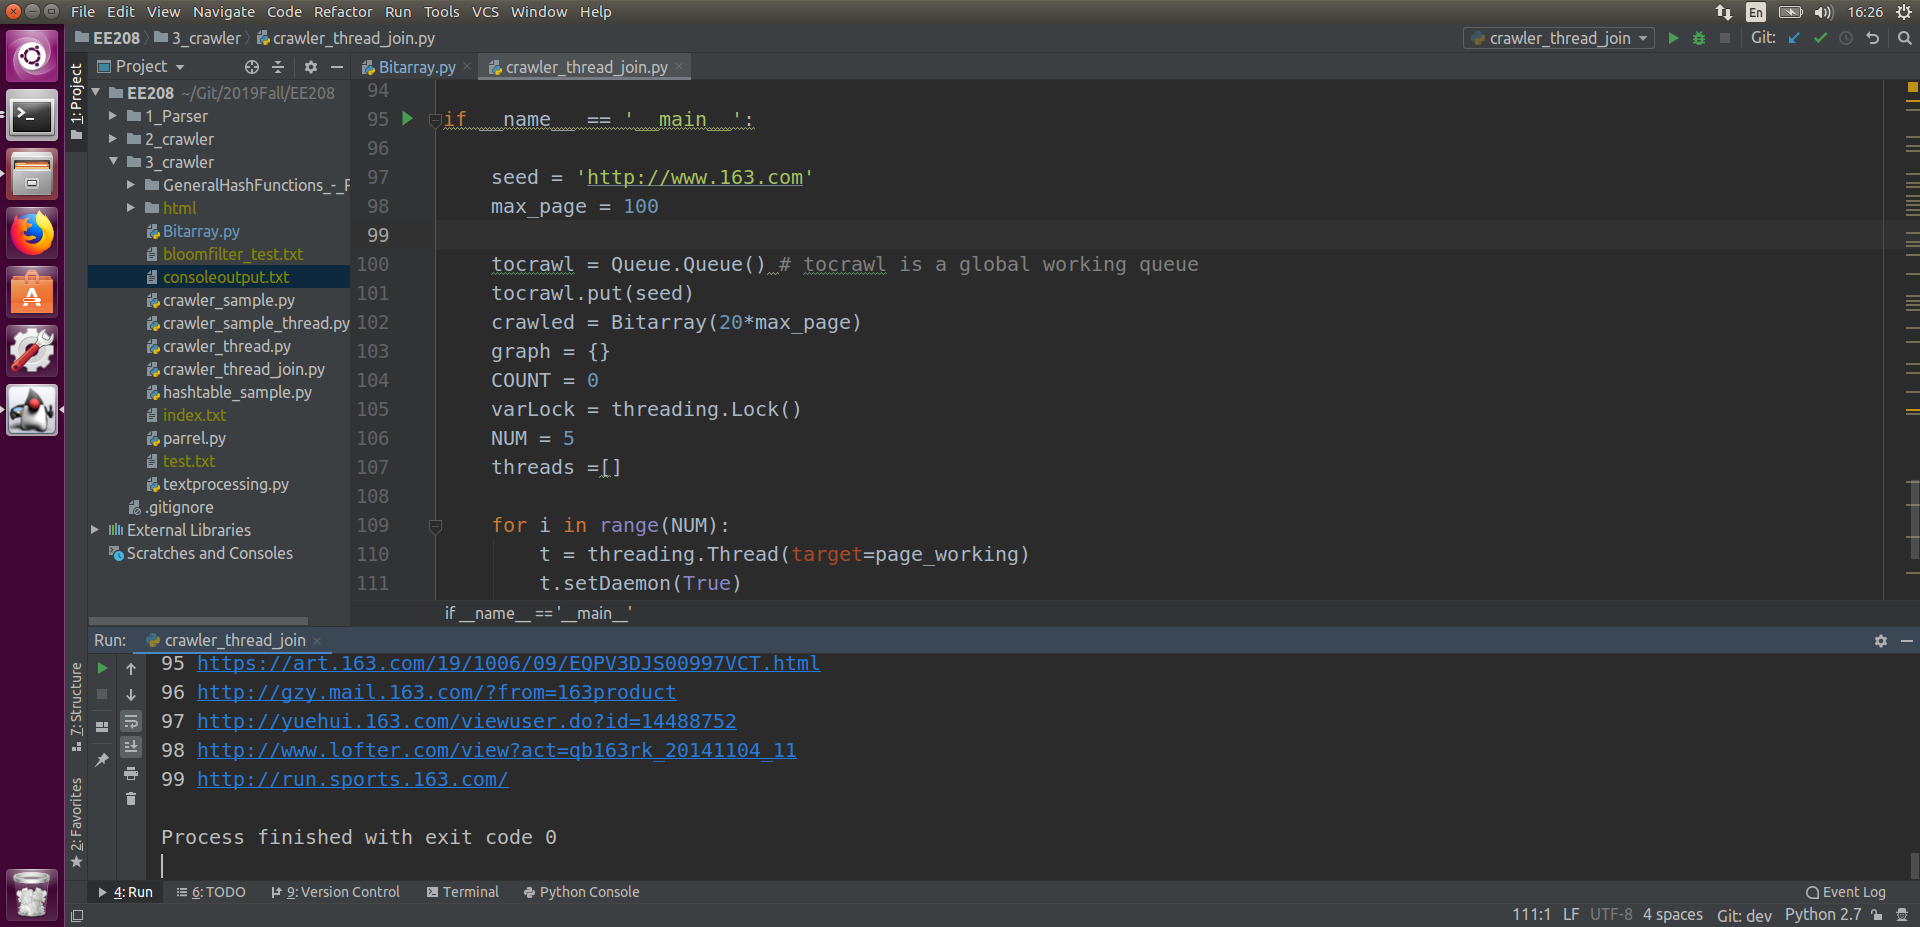
\includegraphics[width=13.5cm]{img/test2.png}
\caption{Crawler Testing}
\label{img:2.1}
\end{figure}


\section{实验总结}
\paragraph{概述}
通过本次实验的学习,我了解了哈希函数的工作原理。通过实现一个BloomFilter的实例和一个并行化爬虫的实例,我学习到了许多优化爬虫项目效率的理论知识和实践技巧。

\paragraph{感想}
在本次实验中,我花了较多的时间在并行化爬虫的搭建上。遇到的主要问题是主函数不能在子线程完成后自动退出。经过反复的试错、排查,我才慢慢理解了什么是工作队列的join()函数,并且认识到对于本实验中到达一定数目后,通过break退出的子线程结构是不适合用工作队列的join函数的,而应该使用线程的join。因此,本次实验带给我的经验是,在实验开始前仔细理解实验原理非常重要,这会减少很多不必要的时间、精力的浪费。

\paragraph{创新}
在本实验中,我将第一部分通过Bitarray类实现的BloomFilter用于了第二部分的crawled集合实现。这一方面进一步提高了并行化爬虫的效率,另一方面也检验了第一部分BloomFilter的实践可行性、可靠性。


\paragraph{问题}
本实验中遇到的主要问题是并行化实现时,join函数无法正常结束主线程。最初我使用了Queue.queue.clear()函数,但经过实践表明仅仅清空队列的元素不能达到标记工作队列任务完成的效果,join函数依然不能通过。随后我写了一个循环,如下所示,在达到目标爬取数,退出循环后,该工作函数中的循环会将剩余队列的所有元素进行批量task\_done()操作,虽然它能保证线程的join成功,但时不时会造成不同线程之间产生冲突报错。

\begin{python}
# 尝试通过批量task_done解决队列的join问题
while True:
    try:
        tocrawl.get()
        tocrawl.task_done()
    except:
        break
\end{python}

经过以上失败的尝试,我意识到队列的join函数是不适合本项目的实现的,因此我改用thread的join函数,既保证了程序能正常退出,也维持了代码的可读性,最终的代码版本在正文中作了详细的阐述。此前失败的尝试可以参考文件crawl\_thread.py或者GitHub上本项目的版本库\href{https://github.com/ltzone/2019Fall/tree/dev/EE208/3_crawler}{\underline{ltzone/2019Fall/EE208/3\_crawler}}。

\end{document}

